\documentclass{article}
\usepackage[utf8]{inputenc}
\usepackage{amsmath}
\usepackage{amssymb}

% \sloppy

\usepackage{authblk}

\usepackage{graphicx}
\usepackage[]{subfigure}
\usepackage{algorithm} 
\usepackage{algpseudocode} 
\usepackage{amsmath}
\usepackage{amssymb}
\usepackage{amsfonts}
\usepackage{xcolor}
% \usepackage{comment}
% \usepackage{nicefrac}
\usepackage{url}
\usepackage{eurosym}
% %\usepackage[normalem]{ulem}
% %\usepackage{showframe} %affiche le page frame pour debugguer
\usepackage{listings}
\usepackage[subtle]{savetrees}

\usepackage{tikz}

% %\usepackage{stmaryrd}
% \newcommand{\llbracket}{[\![}
% \newcommand{\rrbracket}{]\!]}

% \newcommand{\NICOLAS}[1]{{\color{blue}\textbf{NICOLAS:} {#1}}}
% \definecolor{mscolor}{rgb}{0,0.7,0.1}
% \newcommand{\ila}[1]{{\color{mscolor}\textbf{ILARIA:} {#1}}}
% \definecolor{macolor}{rgb}{0.7,0.7,0.1} 
% \newcommand{\MARIYA}[1]{{\color{magenta}\textbf{MARIYA:} {#1}}}
% \definecolor{micolor}{rgb}{0.8,0.2,0.1} 
% \newcommand{\TODO}[1]{{\color{micolor}{#1}}}
% \newcommand{\commentinvisible}[1]{}

% %\newfloat{algorithm}{tbp}{loa}
% %\providecommand{\algorithmname}{Algorithm}
% %\floatname{algorithm}{\protect\algorithmname}

% \usepackage{algorithm}
% \usepackage{algpseudocode}
% \algrenewcommand{\algorithmicrequire}{\textbf{Input:}}
% \algrenewcommand{\algorithmicensure}{\textbf{Output:}}


% %\newtheorem{definition}{Definition}[section]
% %\newtheorem{lemma}{Lemma}[section]
% %\newtheorem{theorem}{Theorem}[section]
% %\newtheorem{corollary}{Corollary}[section]
% \makeatletter
% \newcounter{globalcounter}[section]
% \renewcommand{\theglobalcounter}{\thesection.\arabic{globalcounter}}
% \spnewtheorem{globalenv}[globalcounter]{Dummy}{\bfseries}{\rmfamily}
% \spnewtheorem{assumption}[globalcounter]{Assumption}{\bfseries}{\rmfamily}
% \spnewtheorem{fact}[globalcounter]{Fact}{\bfseries}{\rmfamily}
% \let\c@definition\c@globalenv
% \let\thedefinition\theglobalcounter
% \let\c@lemma\c@globalenv
% \let\thelemma\theglobalcounter
% \let\c@corollary\c@globalenv
% \let\thecorollary\theglobalcounter
% \let\c@theorem\c@globalenv
% \let\thetheorem\theglobalcounter
% \makeatother

% \makeatletter
% %big cdot macro
% \newcommand*\bigcdot{\mathpalette\bigcdot@{.5}}
% \newcommand*\bigcdot@[2]{\mathbin{\vcenter{\hbox{\scalebox{#2}{$\m@th#1\bullet$}}}}}
% \makeatother


% \newcommand{\KeyGen}{\textsf{KeyGen}}
% \newcommand{\Encrypt}{\textsf{Enc}}
% \newcommand{\Decrypt}{\textsf{Dec}}
% \newcommand{\Eval}{\textsf{Eval}}
% \newcommand{\Refresh}{\textsf{Refresh}}
% \newcommand{\LWE}{\mathsf{LWE}}
% \newcommand{\GSW}{\sc{\mathrm{GSW}}}
% \newcommand{\SILWE}{\mathsf{SILWE}}
% \newcommand{\RingLWE}{\sc{\mathrm{RingLWE}}}
% \newcommand{\TLWE}{\sc{\mathrm{TLWE}}}
% \newcommand{\TGSW}{\sc{\mathrm{TGSW}}}
% \newcommand{\LWEPubEncrypt}{\textsf{LWEPubEncrypt}}
% %\newcommand{\LWEDecrypt}{\textsf{LWEDecrypt}}
% \newcommand{\Message}{\textsf{msg}}
% \newcommand{\Error}{\textsf{Err}}
% \newcommand{\Variance}{\textsf{Var}}

% \newcommand{\RingGSW}{\sc{\mathrm{RingGSW}}}
% \newcommand{\SampleExtract}{\textsf{SampleExtract}}
% \newcommand{\KeyExtract}{\textsf{KeyExtract}}

% %gates
% \newcommand{\CMult}{\mathtt{CMult}}
% \newcommand{\Linear}{\mathtt{Linear}}
% \newcommand{\Cst}{\mathtt{Cst}}
% \newcommand{\CAnd}{\mathtt{CAnd}}
% \newcommand{\CMux}{\mathtt{CMux}}
% \newcommand{\Not}{\mathtt{Not}}

% \newcommand{\Bootstrap}{\textsf{Bootstrap}}
% \newcommand{\BK}{\textrm{BK}}
% \newcommand{\cR}{\mathcal{R}}
% \newcommand{\cS}{\mathcal{S}}
% \newcommand{\cM}{\mathcal{M}}
% \newcommand{\cMat}{\mathcal{M}}
% \newcommand{\cN}{\mathcal{N}}
% \newcommand{\bE}{\mathbb{E}}
% \newcommand{\cA}{\mathcal{A}}
% \newcommand{\cL}{\mathcal{L}}
% \newcommand{\cI}{\mathcal{I}}
% \newcommand{\cU}{\mathcal{U}}
% \newcommand{\cX}{\mathcal{X}}
% \newcommand{\cCU}{\mathcal{CU}}





\newcommand{\fT}{\mathfrak{T}}
\newcommand{\fR}{\mathfrak{R}}
\newcommand{\fA}{\mathcal{A}}
\newcommand{\mT}{\mathbb{T}}
\newcommand{\mN}{\mathbb{N}}
\newcommand{\mR}{\mathbb{R}}
\newcommand{\mZ}{\mathbb{Z}}
\newcommand{\mB}{\mathbb{B}}
\newcommand{\bbV}{\mathbb{V}}
\newcommand{\TnX}{\mT_N[X]}


\newcommand{\sergiu}[1]{{\color{red}{\textbf{SERGIU:} {#1}}}}
\newcommand{\nicolas}[1]{{\color{green}\textbf{NICOLAS:} {#1}}}
\newcommand{\mariya}[1]{{\color{pink}\textbf{MARIYA:} {#1}}}
\newcommand{\ila}[1]{{\color{blue}\textbf{ILA:} {#1}}}




\title{IDash 2019 submission}
\author[1]{Sergiu Carpov}
\author[2]{Ilaria Chillotti}
\author[3]{Nicolas Gama}
\author[3]{Mariya Georgieva}
\affil[1]{CEA LIST, Point Courrier 172, 91191 Gif-sur-Yvette Cedex, France}
\affil[2]{imec-COSIC, KU Leuven, Leuven, Belgium}
\affil[3]{Inpher, Lausanne, Switzerland}
\date{August 2019}





\begin{document}

\maketitle

\section{Plaintext version}





\section{Ciphertext version}





\if[0]
\begin{figure}[H]
    \caption{Mux gates}\label{fig:mux}
    \begin{center}
    \includegraphics[width=0.5\textwidth]{figs/mux-full.pdf}
    \end{center}
\end{figure}
\fi

%\vspace{-0.5cm}
\begin{figure}[h]
\caption{Mux gates}\label{fig:mux}
\begin{center}
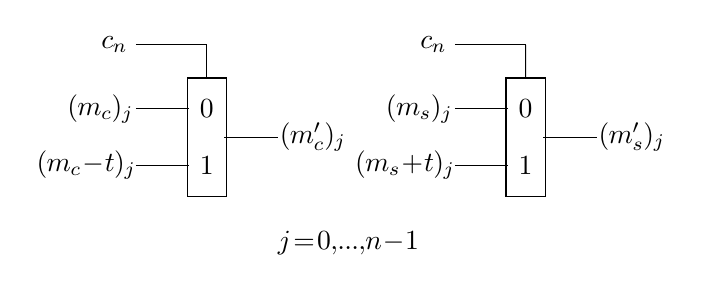
\begin{tikzpicture}[scale=0.9]

\node[draw][minimum width=0.5cm,minimum height=1.5cm] (MUX) at (0,0) {};

\path (0,0.4) node[scale=1]{$0$};
\path (0,-0.4) node[scale=1]{$1$};

\draw[-,>=latex] (-1,1.3) -- (0,1.3);
\draw[-,>=latex] (0,1.3) -- (MUX);
\path (-1.3,1.3) node[scale=1]{$c_n$};

\draw[-,>=latex] (-1,0.4) -- (-0.25,0.4);
\path (-1.5,0.4) node[scale=1]{$(m_c)_j$};

\draw[-,>=latex] (-1,-0.4) -- (-0.25,-0.4);
\path (-1.7,-0.4) node[scale=1]{$(m_c-t)_j$};

\draw[-,>=latex] (0.25,0) -- (1,0);
\path (1.5,0) node[scale=1]{$(m'_c)_j$};
%%%
\node[draw][minimum width=0.5cm,minimum height=1.5cm] (MUX1) at (4.5,0) {};

\path (4.5,0.4) node[scale=1]{$0$};
\path (4.5,-0.4) node[scale=1]{$1$};

\draw[-,>=latex] (3.5,1.3) -- (4.5,1.3);
\draw[-,>=latex] (4.5,1.3) -- (MUX1);
\path (3.2,1.3) node[scale=1]{$c_n$};

\draw[-,>=latex] (3.5,0.4) -- (4.25,0.4);
\path (3,0.4) node[scale=1]{$(m_s)_j$};

\draw[-,>=latex] (3.5,-0.4) -- (4.25,-0.4);
\path (2.8,-0.4) node[scale=1]{$(m_s+t)_j$};

\draw[-,>=latex] (4.75,0) -- (5.5,0);
\path (6,0) node[scale=1]{$(m'_s)_j$};
%%%
\path (2,-1.5) node[scale=1]{$j=0, \ldots, n-1$};
\end{tikzpicture}
\end{center}  
\end{figure}
%\vspace{-0.2cm}


\subsection{Plaintext version}



\begin{algorithm}
\caption{Complex transaction (plaintext algorithm).}
\begin{algorithmic}[1]
    \Require $t$ -- transaction amount (positive or negative)
    \Require $m_0$ -- bank account balance
    \Require $nd_0$ -- old negative days status (number of days negative balance)
    \Require $d$ -- number of days from previous transaction
    \Ensure $s \in \{-1, 0, 1\}$ -- transaction status
    \Ensure $m_1$ -- new bank account balance
    \Ensure $nd_1$ -- new negative days status (number of days negative balance)
    
    \Statex
    
    \State Compute new potential balance: $m_1 = m_0 + t$ \label{algline:new_balance}
    \If{$m_0 < 0$ \textbf{and} $m_1 < 0$} \label{algline:new_negative_status} \Comment{Update negative days status}
        \State $nd_1 = nd_0 + d$ 
    \Else
        \State $nd_1 = 0$
    \EndIf
    
    \Statex
    
    \If{$t < 0$} \Comment{client makes a payment} \label{algline:pay}
        \If{$m_1 < min$ \textbf{or} $nd_1 \geq maxND$}
            \State \Return $(s = -1, m_1 = m_0, nd_1)$ \label{algline:pay-1}
            
        \ElsIf{$m_1 < 0$} \Comment{$m_1 \geq min$ \textbf{and} $nd_1 < maxND$}
            \State \Return $(s = 0, m_1, nd_1)$ \label{algline:pay0}
        \Else \Comment{$m_1 \geq 0$ and $nd_1 = 0$}
            \State \Return $(s = 1, m_1, nd_1 = 0)$ \label{algline:pay1}
        \EndIf

    \Else \Comment{$t \geq 0$, client receives a payment, always allowed} \label{algline:receive}
        \If{$m_1 \geq 0$}
        	\State \Return $(s = 1, m_1, nd_1 = 0)$ \label{algline:receive_positive}
        \Else
            \State \Return $(s = 1, m_1, nd_1)$ \label{algline:receive_negative}
        \EndIf
    \EndIf
    
\end{algorithmic}\label{alg:transactionSenderIdeaClear}
\end{algorithm}








\section{Experimental results}

TFHE~\cite{CGGI18}

\begin{table}[]
    \centering
    \begin{tabular}{c|c|c|c}
        Application & unary (Not) & binary & ternary (Mux) \\
        \hline
        Simple & 35 & 310 & 64 \\
        Complex & 176 & 401 & 32 
    \end{tabular}
    \caption{Gate count in transaction applications.}
    \label{tab:gate_count}
\end{table}


\begin{table}[]
    \centering
    \begin{tabular}{c|c|c|c|c}
        Application & exec. time & RAM usage & input size & output size \\
        \hline
        Simple & 4.9 secs & <200 KB & 189 KB & 128 KB\\
        Complex & 5.1 secs & <200 KB & 189 KB & 131.9 KB
    \end{tabular}
    \caption{Execution performance metrics.% Execution times are given in seconds and memory usage in KB.
    }
    \label{tab:exec_time}
\end{table}



\bibliographystyle{alpha}
\bibliography{biblio}

\end{document}






